%==============================================================================
% Sjabloon poster bachproef
%==============================================================================
% Gebaseerd op document class `a0poster' door Gerlinde Kettl en Matthias Weiser
% Aangepast voor gebruik aan HOGENT door Jens Buysse en Bert Van Vreckem

\documentclass[a0,portrait]{hogent-poster}

% Info over de opleiding
\course{Bachelorproef}
\studyprogramme{toegepaste informatica}
\academicyear{2025-2026} % TODO: controleer of dit klopt met je effectieve academiejaar
\institution{Hogeschool Gent, Valentin Vaerwyckweg 1, 9000 Gent}

% Info over de bachelorproef
\title{Radiogebaseerde Toegang tot een Private Fileserver}
\subtitle{Haalbaarheid en Afstandsgrenzen van een 5,6~GHz SFTP-Verbinding}
\author{Elias Sergoyne}
\email{elias.sergoyne@student.hogent.be}
\supervisor{Peter Beke}
\cosupervisor{Frans Van de Velde}

% Indien ingevuld, wordt deze informatie toegevoegd aan het einde van de
% abstract. Zet in commentaar als je dit niet wilt.
\specialisation{Systeem- en Netwerkbeheer}
\keywords{Radiocommunicatie, SFTP, Point-to-Point, Netwerkemulatie, DFS}
% \projectrepo{https://github.com/TODO/vul-hier-je-eigen-repository-url-in}

\begin{document}

\maketitle

\begin{abstract}
Kan een private fileserver betrouwbaar bereikt worden via een radioverbinding, en tot
welke afstand? Een SFTP-over-5,6~GHz-architectuur werd via netwerkemulatie gebouwd en
over 300 statistische trials getest: geschikt tot ongeveer 15~km.
\end{abstract}

\begin{multicols}{2}

\section{Probleem}

\begin{itemize}
  \item Geen internet op zee, in afgelegen gebieden, bij rampen
  \item Satelliet: te duur, te trage/onbetrouwbare levering
  \item Radioverbindingen: infrastructuuronafhankelijk, weinig onderzocht voor
        \emph{persoonlijke fileservertoegang}
\end{itemize}

\textbf{Onderzoeksvraag:} tot welke afstand werkt een radioverbinding met een private
fileserver betrouwbaar, en onder welke voorwaarden?

\section{Architectuur}

\begin{center}
  \captionsetup{type=figure}
  \includegraphics[width=1.0\linewidth]{../graphics/poster_fig1_test.pdf}
  \captionof{figure}{Server en client, gekoppeld via een point-to-point
  straalverbinding tussen twee antennes.}
\end{center}

\begin{itemize}
  \item \textbf{Protocol:} SFTP (authenticatie + versleuteling, weinig "chatty")
  \item \textbf{Band:} 5,6~GHz, licentievrij (max. 1~W EIRP)
  \item \textbf{Verplicht:} Dynamic Frequency Selection (radar-detectie)
\end{itemize}

\begin{center}
  \captionsetup{type=figure}
  
\includegraphics[width=1.0\linewidth]{../graphics/spectrum_overzicht.pdf}
  \captionof{figure}{Het radiospectrum: bereik en bandbreedte per frequentieband,
  met de DFS-gereserveerde 5~GHz-subbanden.}
\end{center}

\section{Methode}

\begin{itemize}
  \item Fysieke airMAX-hardware niet tijdig beschikbaar $\rightarrow$
        \textbf{volledig gevirtualiseerde} netwerkemulatie (3 VM's, \texttt{tc/netem})
  \item Parameters afgeleid uit officiële productspecificaties
  \item \textbf{Weer:} Gilbert-Elliot-burstverliesmodel (willekeurig per meting)
  \item \textbf{DFS:} stochastische onderbrekingskans, los van afstand
  \item \textbf{3 afstandscategorieën} $\times$ 100 trials = 300 metingen
  \item Volledig geautomatiseerd: enkele dubbelklikbare Windows-scripts
\end{itemize}

\section{Resultaten}

\begin{center}
  \captionsetup{type=figure}
  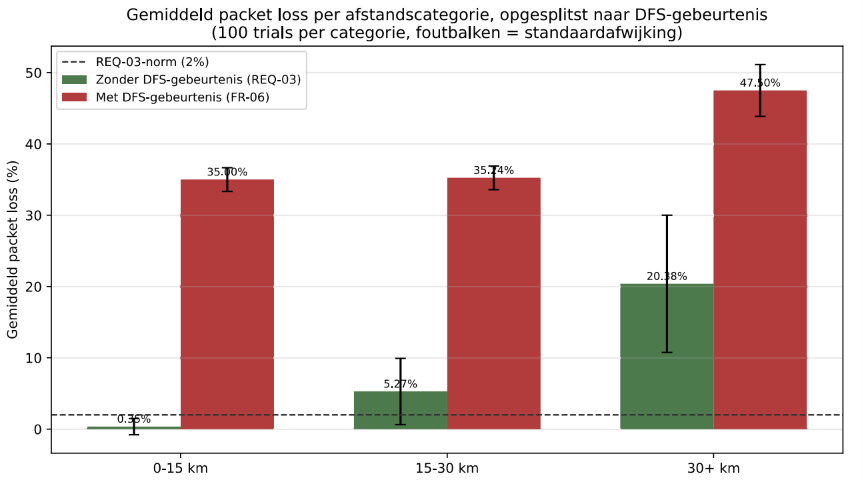
\includegraphics[width=1.0\linewidth]{../graphics/packetloss_per_afstand.pdf}
  \captionof{figure}{Gemiddeld packet loss per afstandscategorie. Groen: normale
  werking. Rood: tijdens een DFS-onderbreking. Stippellijn: norm van 2\%.}
\end{center}

\begin{itemize}
  \item \textbf{0--15~km:} 0,35\% verlies -- ruim binnen de norm
  \item \textbf{15--30~km:} 5,27\% -- norm structureel overschreden
  \item \textbf{30+~km:} 20,38\% -- vrijwel altijd overschreden
  \item DFS-herstel werkt betrouwbaar op \textbf{elke} afstand
\end{itemize}

\section{Conclusie}

\begin{itemize}
  \item Radiogebaseerde fileservertoegang: haalbaar tot \textbf{$\pm$15~km}
  \item Geen harde grens, maar een geleidelijke overgang
  \item Herbruikbare, statistisch onderbouwde testmethodologie
\end{itemize}

\textbf{Vervolgonderzoek:} fysieke veldvalidatie, gelicentieerd spectrum, multi-hop
relais, gemeten (i.p.v.\ geschatte) weersdata.

\end{multicols}
\end{document}